\begin{figure}[h]
    \centering
    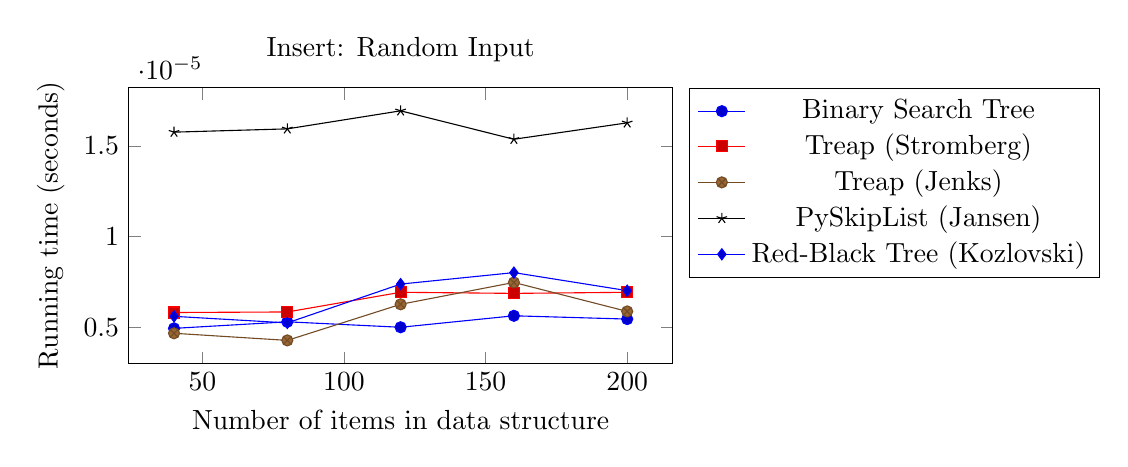
\begin{tikzpicture}
        \begin{axis}[
            xlabel={Number of items in data structure},
            ylabel={Running time (seconds)},
            title={Insert: Random Input},
            width=0.7\textwidth,
            height=2in,
            legend pos=outer north east
        ]
		\addplot coordinates {
			(40, 4.939275522727882e-06)
			(80, 5.300685926828974e-06)
			(120, 4.9995105900785266e-06)
			(160, 5.63197879725752e-06)
			(200, 5.451273595205586e-06)
		};
		\addplot coordinates {
			(40, 5.812683999306678e-06)
			(80, 5.842801532982e-06)
			(120, 6.9270327452880535e-06)
			(160, 6.866797677937409e-06)
			(200, 6.9270327452880535e-06)
		};
		\addplot coordinates {
			(40, 4.668217719652757e-06)
			(80, 4.276689781873566e-06)
			(120, 6.264447004436513e-06)
			(160, 7.469148351443855e-06)
			(200, 5.872919066657323e-06)
		};
		\addplot coordinates {
			(40, 1.5751470112113086e-05)
			(80, 1.5932175314162245e-05)
			(120, 1.6926053925445107e-05)
			(160, 1.535994217433667e-05)
			(200, 1.626346818459079e-05)
		};
		\addplot coordinates {
			(40, 5.601861263579422e-06)
			(80, 5.240450859481105e-06)
			(120, 7.378795750415113e-06)
			(160, 8.011263957594106e-06)
			(200, 7.0173853463140205e-06)
		};
        \legend{Binary Search Tree, Treap (Stromberg), Treap (Jenks), PySkipList (Jansen), Red-Black Tree (Kozlovski)}
        \end{axis}
    \end{tikzpicture}
    \caption{Average of 10 operations, benchmarked every 40, starting at 40.}
\end{figure}